\chapter{Scenarios and user stories}

From the previous personas, scenarios were developed to clarify what the personas expectations for the extension could be.
\begin{quote}
``A scenario is a story adapted and structured for engineering use. The purpose of a scenario is to communicate a situation (...) in a series of steps.''  
\end{quote} \citep[98]{scenario}
Based on the scenarios below, the following user stories could be identified. \\
\\
The user stories follow the style of the Connextra development team (\textit{Connextra format}), which is
\begin{quote}
\textit{As a [user role], \newline I want [function], \newline So that[benefit]}
\end{quote} 
\citep{connextrastory,userstory}
The user stories are part of every scenario and important to identify the following non-functional and functional requirements because they abstract from the scenarios. 

\section{Scenario Rashidi}
Rashidi listens to Jazz on the radio. He loves Louis Armstrong, and wants to find more information about him. He uses \textit{Google} to look up Louis Armstrong and arrives at the ArticlePlaceholder on Hausa Wikipedia. There he can read up Louis Armstrong's date of birth (\textit{4 August 1901}), place of birth (\textit{New Orleans}) \citep{wd:03}, and can get more information on New Orleans, for example, to learn that New Orleans is a city in the United States of America. 
\begin{figure}[H]
	\centering
	\includegraphics[width=\textwidth]{diagrams/UserDiagramRashidiArmstrong.png}
	\caption{Scenario Rashidi}
	\label{fig:ScenarioRashidi}
\end{figure}

\paragraph{User stories Rashidi} ~\\
As a reader of a small Wikipedia, I want to access all information available in my language, so that I can use my Wikipedia without disadvantages. \\
\\
As a reader of a Wikipedia, I want to search for a topic and get all information available even if there is no article created yet, so that I can read up on the topic. \\
\\
As an editor and reader of a very small Wikipedia, I want to have a pleasant layout of any content page, so that I do not have to adjust to new styles.

\section{Scenario Edha} 
Edha talks with friends about an exhibition they have been to. She hears about Rembrandt, a Dutch painter. As soon as she gets home she realizes she forgot to ask what century he lived in, and where in the Netherlands he was born. She wants to look up the information on Wikipedia in her own language. \\
\\ 
She opens Wikipedia on her phone and enters ``Rembrandt'' in the searchbar. Because there is no article on Rembrandt yet, she finds the ArticlePlaceholder for \textit{``Rembrandt'' (Q5598)} \citep{wd:01} in the results page. Since it also displays the description of the item (\textit{Dutch 17th century painter and etcher}) on the search page next to the name of the painter, she can validate with that description that she has found the right information. \\
She gets an overview of Rembrandt on the page, and can find the place of birth on the ArticlePlaceholder, which is \textit{Leiden}. She has not heard of the place and searches for it on Wikipedia again. She finds the description \textit{city and municipality in South Holland, Netherlands} \citep{wd:02} already on the search page. That is the information she was looking for, so she goes back to the ArticlePlaceholder. Since in the meantime someone has edited the item on Wikidata, she now finds even more information about him on the ArticlePlaceholder. It also tells her that his date of birth is \textit{15 July 1606} \citep{wd:01}. \\
\\
In the next few days she researches more on Rembrandt in her local library. With this additional information she decides to create an article. She goes back to the ArticlePlaceholder to get some of the information and references already there. Then she clicks the button \textit{create an article}, which is labeled in her language. She is able to add the title for the page, which is translated \textit{Rembrandt (painter)} in English to make clear which Rembrandt she means. This title differs from the title of the ArticlePlaceholder, which is only \textit{Rembrandt}. She can then enter the information she has gathered, and create an actual article. She would have the option to translate the article from English, too, but decides to prefers to create a new article.
\begin{figure}[H]
	\centering
	\includegraphics[width=\textwidth]{diagrams/UserDiagramEdhaRembrandt.png}
	\caption{Scenario Edha}
	\label{fig:ScenarioEdha}
\end{figure}

\paragraph{User stories Edha} ~\\
As a reader of a small Wikipedia, I want any content page to work on every device independently of screen size, so that I can access Wikipedia everywhere. \\
\\
As an editor, I want to have the option to translate articles from an ArticlePlaceholder, so that I am able to contribute to the diversity of articles on my Wikipedia. \\
\\
As an editor, I want to have an easy way to get from an ArticlePlaceholder to the edit page, so that I can create an article when appropriate. 

\section{Scenario Julian}
Julian has heard that ArticlePlaceholder has been enabled on German Wikipedia. But since this Wikipedia has quite a lot of articles, he is aware that he will seldomly need it. \\
As part of a presentation in school, he wants to research \textit{KDE e.V.}. He searches for it on Wikipedia and gets to the ArticlePlaceholder. He uses the data references provided there. \\
He dislikes the way the data is displayed though, and wants to adjust the layout. He has contributed to a module before, so he knows how to write Lua code. He wants to overwrite one of the functions. After a discussion with the local community, who support Julian's changes, he adds the code after testing it, and the ArticlePlaceholder is adjusted to the community's needs.

\begin{figure}[H]
	\centering
	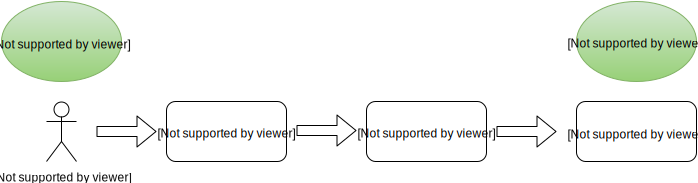
\includegraphics[width=\textwidth]{diagrams/UserDiagramJulianLua.png}
	\caption{Scenario Julian}
	\label{fig:ScenarioJulian}
\end{figure}

\paragraph{User stories Julian} ~\\
As an editor familiar with Lua, I want to be able to adjust the layout of the ArticlePlaceholder on my Wikipedia, so that I can adjust it to the needs of my community. \\
\\
As an editor, I want to influence the order in which information is shown in, so that I can adapt it to what is most important for my community. An order which may differ from that of other communities.

\section{Scenario Catrin}
One of Catrin's students tells her he was born in \textit{Kasımpaşa}. She has never heard of it and back at home she wants to research it on French Wikipedia. She enters the term in the search bar. Since there is no article on the French Wikipedia, she gets to an ArticlePlaceholder. It has no description, so she can only see the name. She learns it is an \textit{instance of neighborhood} and is \textit{located in the administrative territorial entity Beyoğlu}. Since she has not heard of Beyoğlu yet either, she continues her research and gets to the French Wikipedia article Beyoğlu. There she finds out Beyoğlu is a district of Istanbul, Turkey.
\begin{figure}[H]
	\centering
	\includegraphics[width=\textwidth]{diagrams/UserDiagramCatrinKasimpase.png}
	\caption{Scenario Catrin}
	\label{fig:ScenarioCartin}
\end{figure}

\paragraph{User stories Catrin} ~\\
As a reader, I want to see the most important information on a page first, so that I do not have to read through everything to get to what really interests me. \\
\\
As a reader, I want to be able to clearly differentiate between a generated content page and a manually written article, so that I can classify the information in the appropriate context.

\section{Scenario Heather}
Heather has worked on the Wikidata item \textit{``Ada Lovelace'' (Q7259)} over the last few days. She has added data and references mostly by hand. She wants to see what the item would look like on a Wikipedia that does not have an article on \textit{Ada Lovelace} yet. \\
She is involved with various small language Wikipedias and even though she does not speak the language, she can find the SpecialPage, which will bring her to an ArticlePlaceholder, and enters the item ID there to see what it looks like. \\
When she enters the same item ID on English Wikipedia, she is redirected to the existing article on \textit{Ada Lovelace}.
\begin{figure}[H]
	\centering
	\includegraphics[width=\textwidth]{diagrams/UserDiagramHeatherSmallWP.png}
	\caption{Scenario Heather, small Wikipedia}
	\label{fig:ScenarioHeatherSmall}
\end{figure}
\begin{figure}[H]
	\centering
	\includegraphics[width=\textwidth]{diagrams/UserDiagramHeatherEnWiki.png}
	\caption{Scenario Heater, English Wikipedia}
	\label{fig:ScenarioHeatherEnWiki}
\end{figure}

\paragraph{User stories Heather} ~\\
As a reader familiar with Wikidata, I want to see the ArticlePlaceholder of a certain item, so that I can link to the placeholder rather than the Wikidata item. \\